\section{Outils}
 \subsection{Spring}
 
  \subsubsection{Spring Framework }
  
  
  Spring Framework fournit un modèle complet de programmation et de configuration pour les applications d'entreprise modernes basées sur Java - sur tout type de plate-forme de déploiement.
  
  Un élément clé de Spring est le support infrastructurel au niveau de l’application: Spring met l’accent sur la «plomberie» des applications d’entreprise afin que les équipes puissent se concentrer sur la logique métier au niveau de l’application, sans liens inutiles avec des environnements de déploiement spécifiques.
  
 \subsubsection{Spring boot}
 Spring Boot makes it easy to create stand-alone, production-grade Spring based Applications that you can "just run".
 
 We take an opinionated view of the Spring platform and third-party libraries so you can get started with minimum fuss. Most Spring Boot applications need very little Spring configuration.
   \subsubsection{Spring Data}
   
 \subsubsection{Spring Cloud}
 Spring Cloud fournit aux développeurs des outils permettant de créer rapidement certains modèles courants dans les systèmes distribués (gestion de la configuration, découverte de services, disjoncteurs, routage intelligent, micro-proxy, bus de contrôle, jetons à usage unique, verrous globaux, élection des dirigeants, distribution sessions, état du cluster). La coordination des systèmes distribués conduit à des modèles de plaque de chaudière et, grâce à Spring Cloud, les développeurs peuvent rapidement mettre en service des services et des applications mettant en œuvre ces modèles. Ils fonctionneront bien dans n’importe quel environnement distribué, y compris l’ordinateur portable du développeur, les centres de données à nu et les plateformes gérées telles que Cloud Foundry.
 
 
  \subsubsection{Spring Cloud Netflix}
 Spring Cloud Netflix fournit des intégrations Netflix OSS pour les applications Spring Boot via la configuration automatique et la liaison à Spring Environment et à d'autres idiomes de modèles de programmation Spring. Quelques annotations simples vous permettent d'activer et de configurer rapidement les modèles courants dans votre application et de créer de grands systèmes distribués avec des composants Netflix testés au combat. Les modèles fournis incluent la découverte de service (Eureka), le disjoncteur (Hystrix), le routage intelligent (Zuul) et l’équilibrage de la charge côté client (ruban).
 
 \subsection{ Qu'est-ce que Micro Service?}

 L'objectif principal de la mise en œuvre des micro-services est de scinder l'application en un service distinct pour chaque fonctionnalité de base et chaque service de l'API. Elle devrait être déployée indépendamment sur le cloud. Nous avons choisi le langage de programmation réactif du projet familial spring.io avec un ensemble de composants pouvant être utilisés pour mettre en œuvre notre modèle d'exploitation. Spring Cloud intègre très bien les composants Netflix dans l’environnement Spring. Il utilise une configuration automatique et une convention de configuration similaire à celle du fonctionnement de Spring Boot.


\subsubsection{Pourquoi l’architecture de Microservices?}

Nous avons choisi l'architecture de micro-services pour écrire chaque fonctionnalité en tant que service distinct pour les fonctionnalités de base et d'API, ce qui nous aide à réaliser la livraison et l'intégration en continu.

\subsubsection{Patterns dans l'architecture des microservices}



\begin{itemize}
\item  \textbf{Api Gatway }


\begin{enumerate}
	
\item 	  Choisissez de créer l’application en tant qu’ensemble de micro-services.

\item	  Décidez comment le client de l'application va interagir avec les micro-services.

\item	  Avec une application monolithique, il n'y a qu'un seul ensemble de points d'extrémité (généralement répliqués, à charge équilibrée).

\item	  Dans une architecture de micro-services, chaque micro-service expose cependant un ensemble de
points finaux.
\end{enumerate}


\item \textbf{Service registry}

\begin{enumerate}
\item 	  Le registre de service aide à déterminer l’emplacement des instances de service pour envoyer la demande au correspondant
	un service
	
\item 	  Ici, nous avons utilisé Netflix Eureka pour enregistrer un service pouvant être enregistré dans le registre de services.
	serveur et il peut être identifié par le routeur.

	
\end{enumerate}
\item \textbf{Service Discovry}
\begin{enumerate}


\item   Dans une application monolithique, les services s'appellent par le biais d'appels de méthode ou de procédure au niveau de la langue.

\item   Toutefois, dans une application moderne basée sur des micro-services, elle s'exécute généralement dans des environnements virtualisés où le nombre
des instances d'un service et de leurs emplacements change de façon dynamique.

\item   Chaque service peut être identifié à l'aide d'un routeur enregistré auprès du serveur de registre de services.
	
\end{enumerate}
\end{itemize}






\subsubsection{Architecture des microservices via les composants Netflix}
Nous avons utilisé les composants Netflix pour réaliser les modèles d’architecture de microservices ci-dessus.

% Please add the following required packages to your document preamble:
% \usepackage[table,xcdraw]{xcolor}
% If you use beamer only pass "xcolor=table" option, i.e. \documentclass[xcolor=table]{beamer}
% \usepackage[normalem]{ulem}
% \useunder{\uline}{\ul}{}
\begin{table}[H]
	\begin{tabular}{|l|l|}
		\hline
		\rowcolor[HTML]{5174DA} 
		{\color[HTML]{FFFFFF} \textbf{Operations Component}} & {\color[HTML]{FFFFFF} \textbf{Spring, Netflix OSS}} \\ \hline
		Service Discovery server & Netflix Eureka \\ \hline
		Edge Server & Netflix Zuul \\ \hline
		Central configuration server & Spring Cloud Config Server \\ \hline
		Dynamic Routing and Load Balancer & Netflix Ribbon \\ \hline
		OAuth 2.0 protected API’s & Spring Cloud + Spring Security OAuth2 \\ \hline
		Monitoring & Netflix Hystrix dashboard and turbine \\ \hline
	\end{tabular}
\end{table}

\subsection{Composantes majeures de Netflix}



\subsubsection{Service Discovery Server} 

\authorimg{images/ms-img04} Netflix Eureka permet aux micro-services de s’enregistrer eux-mêmes au moment de leur exécution, tels qu’ils apparaissent dans la structure du système.



\subsubsection{Routage dynamique et équilibreur de charge} 

\authorimg{images/ms-img05}  Netflix Ribbon peut être utilisé par les consommateurs de services pour rechercher des services au moment de l’exécution. Le ruban utilise les informations disponibles dans Eureka pour localiser les instances de service appropriées. Si plusieurs instances sont trouvées, le Ruban appliquera un équilibrage de charge pour répartir les demandes sur les instances disponibles. Le ruban ne s'exécute pas en tant que service distinct, mais en tant que composant intégré dans chaque consommateur de service.





\subsubsection{Serveur Edge} 

\authorimg{images/ms-img06}  Zuul est (bien sûr) notre gardien du monde extérieur, ne permettant pas le passage de demandes externes non autorisées. Zulu fournit également un point d'entrée bien connu aux micro-services dans le paysage système. L'utilisation de ports alloués de manière dynamique est pratique pour éviter les conflits de ports et minimiser l'administration, mais elle rend évidemment la tâche plus difficile pour tout consommateur de services donné. Zuul utilise Ribbon pour rechercher les services disponibles et achemine la demande externe vers une instance de service appropriée.


\subsection{Spring Boot et Spring Cloud Netflix OSS – Micro Service Architecture}

\subsubsection{Micro Services avec Spring Boot}

 

Spring Boot est un tout nouveau framework de l'équipe de Pivotal, conçu pour simplifier le démarrage et le développement d'une nouvelle application Spring. Le cadre adopte une approche de configuration avisée, libérant les développeurs de la nécessité de définir la configuration standard.

\subsubsection{Spring Cloud Netflix}
 

Spring cloud Netflix fournit des intégrations Netflix OSS pour les applications de démarrage printanier via la configuration automatique et la liaison à l'environnement Spring et à d'autres modèles de programmation Spring. Avec quelques annotations simples, nous pouvons rapidement activer et configurer des modèles courants dans une application et construire des systèmes distribués volumineux avec des composants Netflix. De nombreuses fonctionnalités sont disponibles avec le nuage de printemps Netflix. Ici, nous avons répertorié certaines des fonctionnalités communes que nous avons implémentées avec les micro-services avec Spring Boot et Netflix,

\begin{itemize}
\item \textbf{Découverte du service:}
	
	Les instances Eureka peuvent être enregistrées et les clients peuvent
	Découvrez les exemples à l'aide de haricots à gestion printanière
	

\item \textbf{	Création de service:}	
	Le serveur Eureka intégré peut être créé avec
	configuration Java déclarative
	
\item \textbf{	Configuration Externel:}	
	
	Bridge from the Spring Environment (permet aux utilisateurs de
	configuration des composants Netflix à l'aide de Spring Boot
	conventions)
	
      \item \textbf{	Routeur et filtre:}	
	
	Enregistrement automatique des filtres Zuul, et un simple
	convention sur l'approche de configuration pour la création de proxy inverse.
\end{itemize}
 
 \section{Conception:}
 \subsection{Diagramme de Classe}
 \begin{figure}[H]
 	\centering
 	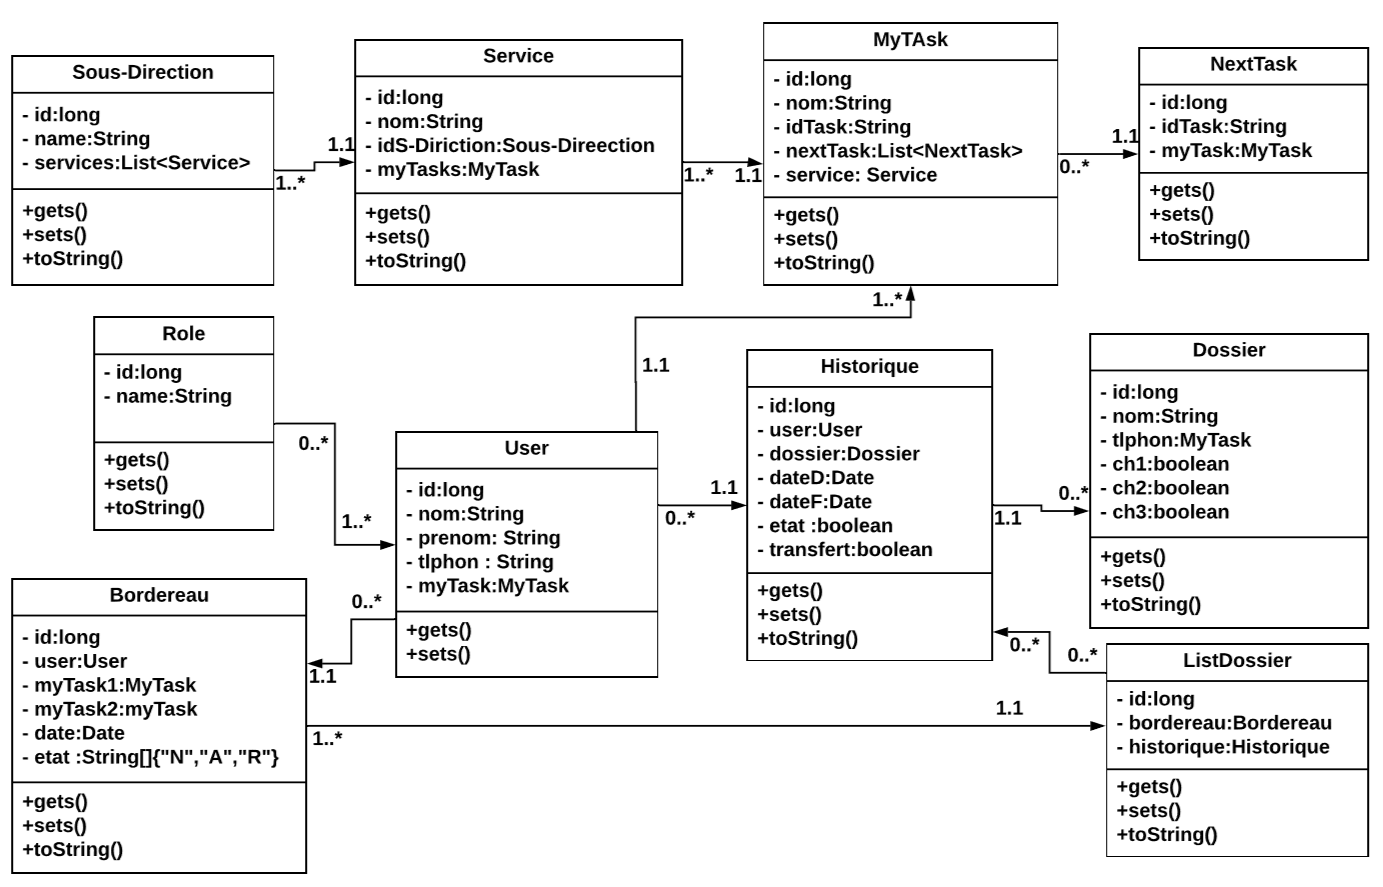
\includegraphics[width=1\linewidth]{images/class3}
 	\caption{Diagramme de Classe}
 	\label{fig:class}
 \end{figure}
   